\chapter{Goals} \label{chap:goals}

Systems such as Qubes OS, Bromium and Chrome are successful in preventing attacks that exploit software bugs. However, their security guarantees are insufficient to prevent phishing attacks. In this chapter, we list the properties of an ideal secure workstation. We also list attack scenarios that the workstation would be able to prevent.

\paragraph{Blocking malicious content:} The primary property of a secure workstation is the ability to block malicious content. Malicious content can be accessed by users in various ways: the website the user is visiting may have been compromised, malicious content could have been posted by an attacker on a public forum, or users may explicitly navigate to a malicious website. The system must take steps to identify such content and block it from being displayed.

\paragraph{Unambiguous User Interface:} A lot of phishing attacks operate by displaying a fake login page to the user. A secure workstation must ensure that the user can only enter sensitive information in genuine websites, and have mechanisms to defend against fake websites.

\paragraph{Damage Containment:} Even after taking several precautions, some damage is inevitable. We cannot foresee all sorts of future attacks that may come up. The secure workstation must ensure that in the unlikely event of a malicious software being able to execute, the damage caused is contained. The risk of leaking sensitive information in such events must be minimized.

The rest of this chapter focuses on case studies to make the goals of the secure workstation more concrete.

\section{Blocking Malicious Content}

Several phishing attacks operate by including malicious content in places which appear to come from legitimate sources. This content can include malicious software, fake login pages, etc. Below we list two phishing scenarios which highlight ways these attacks operate.

\paragraph{Fake Gmail Attachment Scam: }
The first case we look at is a phishing email scam \cite{fake-attachment-scam} which uses fake attachments in order to lure the users into clicking on it. The email has an image of what looks like a Gmail attachment but in-fact is a link to an external page. Figure~\ref{fig:fake-attachment} shows how the email appears to the user.

\begin{figure}[p]
\centering
    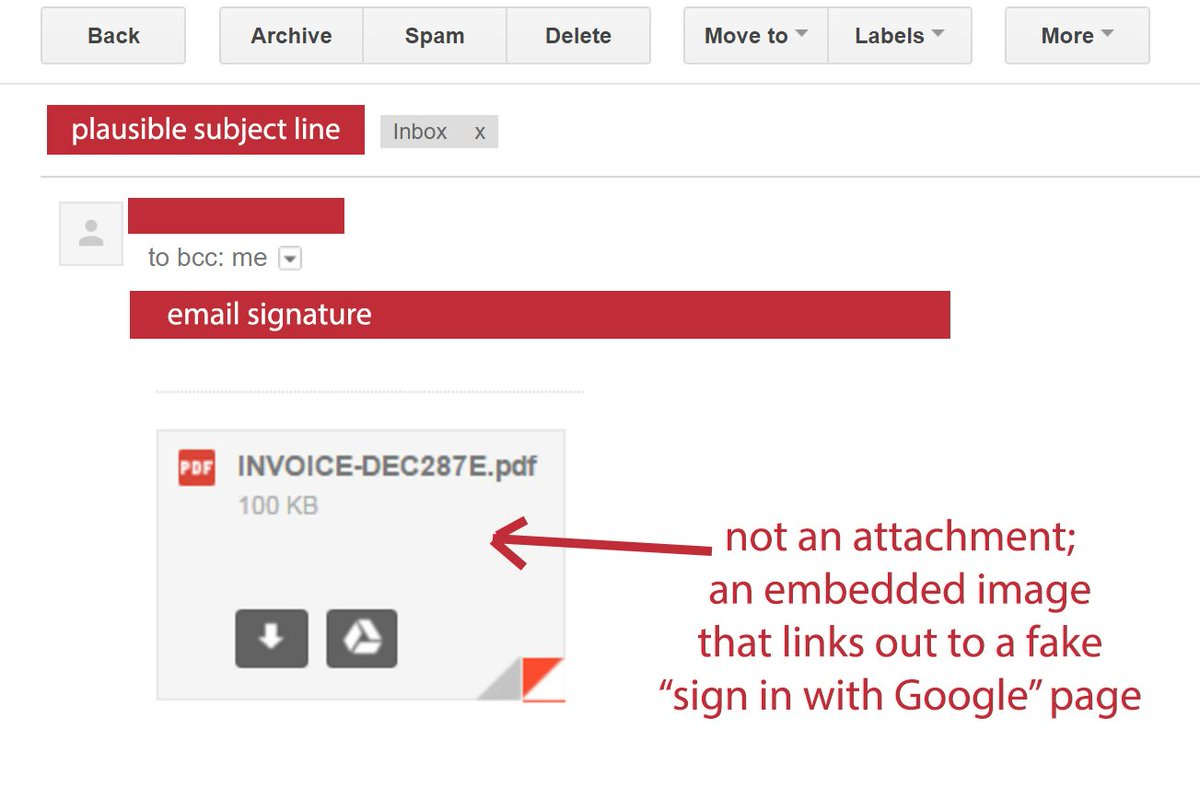
\includegraphics[width=1.0\textwidth]{tomscott-gmail-phishing.jpg}
    \caption{The email in this figure has an image which appears to be an attachment but in-fact is a link to an external page which displays a login page.}
   \label{fig:fake-attachment}
\end{figure}

Figure \ref{fig:fake-attachment-login} shows the page displayed when the user clicks on the fake attachment link. This page shows several other features that are common among phishing attacks such as a deceptive URL, similar looking Google login page, missing SSL/TLS certificates which would identify this page as belonging to Google, etc. The attackers can steal the credentials that the users enters on this page.

\begin{figure}[p]
\centering
    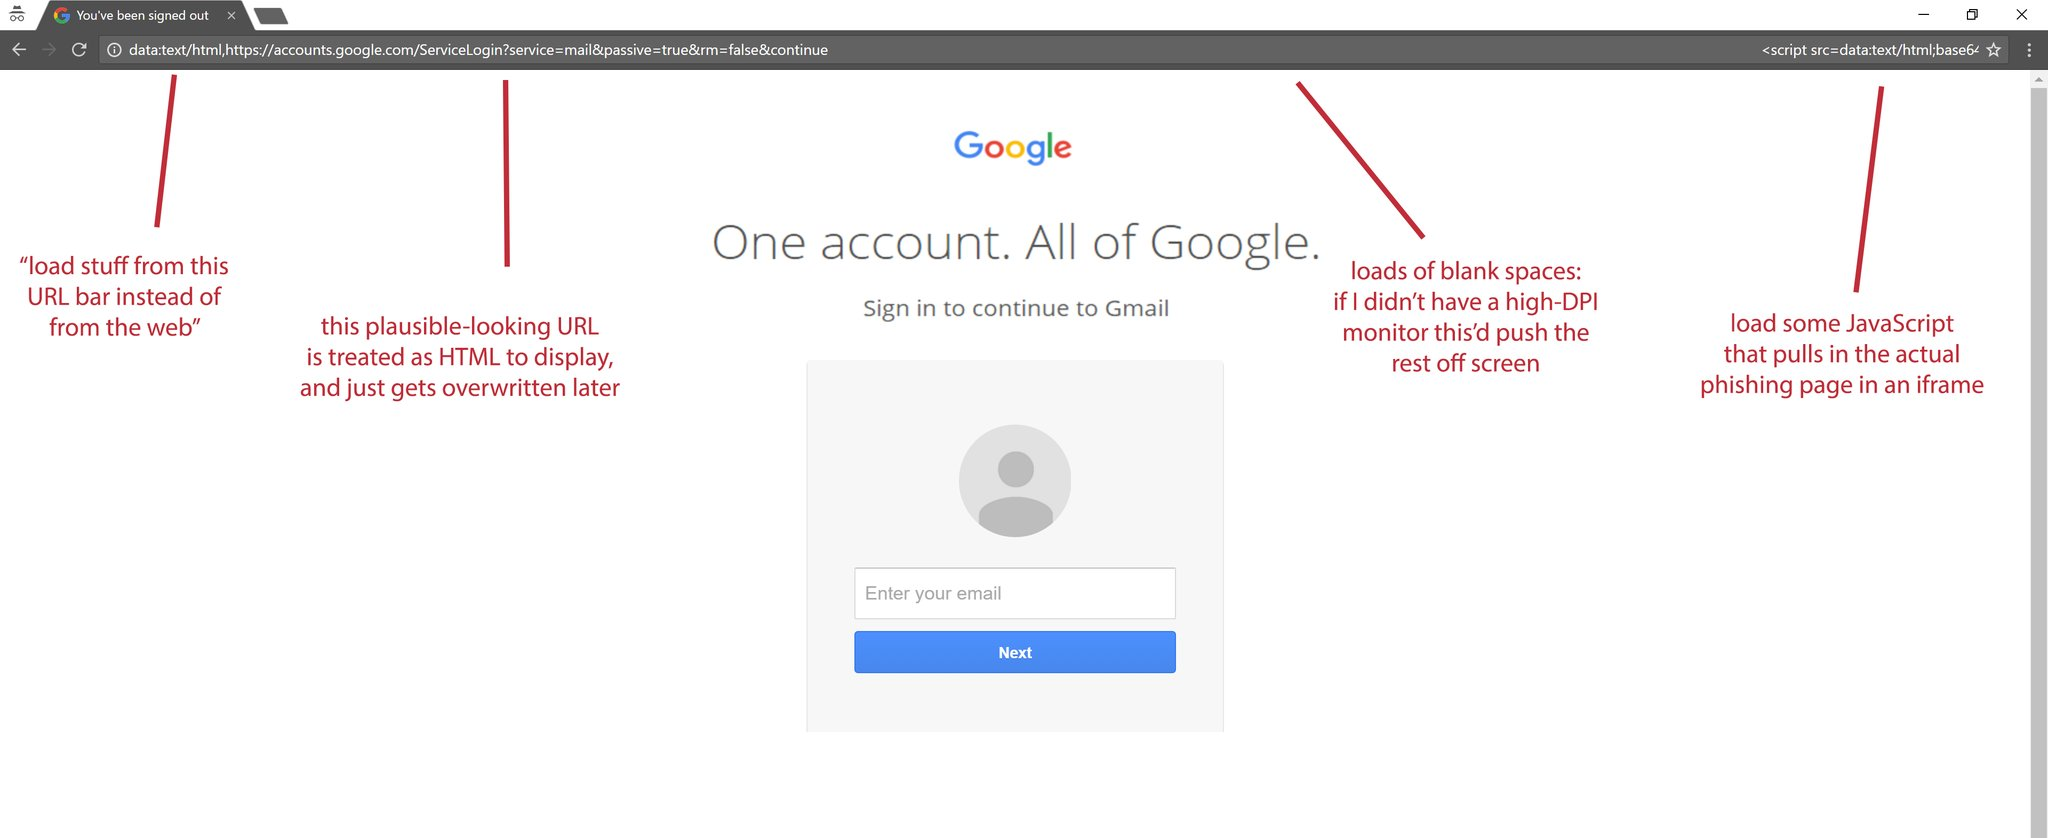
\includegraphics[width=1.0\textwidth]{tomscott-gmail-login.jpg}
    \caption{Clicking on the fake attachment leads to this fake login page.}
   \label{fig:fake-attachment-login}
\end{figure}

There were other ways this attack could have worked. The attachment link could have led to an external URL which would have download a malicious software into the user's computer. A secure workstation must be able to defend against such attacks. It should include mechanisms to avoid displaying such links, stopping the download of malicious software or prevent users from getting tricked into entering credentials into fake login pages.

\paragraph{Malvertising:} The second case we analyze is of malvertising \cite{malvertising}, malicious advertisements displayed on legitimate websites. Consider a recent attack \cite{malvertisement-nytimes} that used malvertisements on major news outlets like New York Times, BBC, etc. Attackers were able to inject malicious software in legitimate online ad networks. When users visited the website, it would redirect them to the attackers website which would target security holes in software such as Microsoft Silverlight and Adobe Flash. If the compromise was successful, a ransomware would get installed and encrypt the users files.

A major factor responsible for the success of this attack was that the news outlets trusted the external ad services into displaying anything in their webpages. There was no protection that in the unlikely event these services get compromised, the outlet websites do not get affected. A secure workstation must be able to defend against such attacks by including mechanisms to restrict the trust placed in externally linked content.

In summary, for a workstation to be secure against malicious content, it should have the following properties:

\begin{itemize}
    \item Mechanisms to \textbf{block malicious content} to be displayed in the first place,
    \item Methods to identify and \textbf{differentiate genuine content from malicious content}, and
    \item \textbf{Fallback mechanisms} in case of a compromise in a subsystem.
\end{itemize}

\section{Unambiguous User Interface}

Exploiting the user interface is another mechanism through which phishing attacks operate. The main goal of phishing attacks is to trick the user into believing the phishing content to be genuine. We analyze some of these ways below.

\paragraph{Faking other websites:} Some phishing websites operate by appearing to be a duplicate of a genuine website. Some may even have similar looking domains names. These websites usually present a login form to the user where the user is tricked into entering their credentials. Upon submitting the login form, the attackers can steal their credentials and optionally redirect the user to the genuine login form. The user is lead to believe they have mistakenly typed their password incorrectly and they are none the wiser.

As an example, consider the case of the usage of Punycode in browsers. As the world is adopting Unicode, it is possible to use any Unicode characters in browsers. To encode non-ASCII characters, browsers use a encoding called Punycode. A recent vulnerability \cite{punycode-attack} discovered takes advantage of the encoding of similar looking characters to display websites whose domain name appears visually indistinguishable from real domain names. Further, it is possible to also obtain free SSL/TLS certificates for the fake domain names. The only way for the user to tell the difference between a real and a fake website is then to explicitly check the certificate. For example, domains names can use both a Unicode Cyrillic small letter ``a" or a Latin small letter ``a". Both look visually indistinguishable. We can encode the domain {\tt apple.com} using alternative characters in Punycode as {\tt xn--80ak6aa92e.com}. When shown in browser, both domains appear identically as {\tt apple.com}. Figure~\ref{fig:punycode-apple} shows how both domains appear in the browser.

\begin{figure}[p]
\centering
    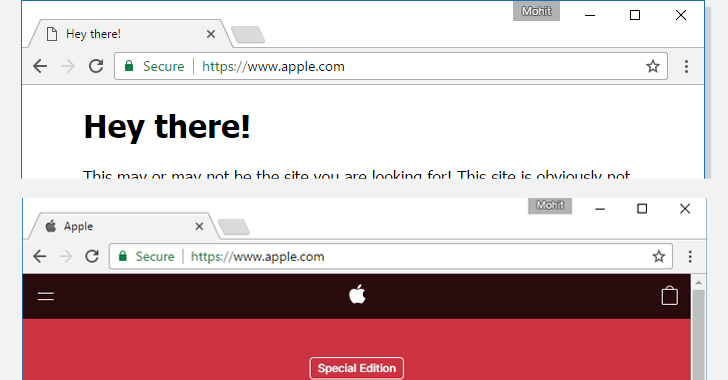
\includegraphics[width=1.0\textwidth]{punycode-apple}
    \caption{Both domain names are similar except their use of the small letter ``a". One uses a Unicode Cyrillic ``a" whereas the other uses a Latin ``a".}
   \label{fig:punycode-apple}
\end{figure}

A secure workstation must be able to mitigate such attacks by including mechanisms to verify that the website the user is visiting is the website the user intended to visit.

\paragraph{Faking system prompts:} Another common way that phishing attacks operate is by showing fake system prompts. One popular attack works by showing a fake prompt to the user displaying that the user's computer is infected and asking them to click on a link to download an antivirus software. The link in reality downloads a malicious software to compromise the user's computer.

A secure workstation must have mechanisms to let the user distinguish between content displayed by the system and content displayed by the website. It must \textbf{provide ways to distinguish fake and genuine content}.

\section{Damage Containment}

Even after taking all the precautions, it is still very hard to stop all kinds of attacks. Thus it is important to plan how a secure workstation would handle a compromised system. The primary principle to be followed in case of a security breach should be to contain the damage as much as possible. For example, if a webpage gets compromised no other webpages should be affected, or if a browser instance gets compromised no other browser instances should be affected.

We will analyze the case of ransomware attacks to understand why damage containment is important even after the system gets compromised. A ransomware software needs to be first executed on a system to take effect. It can be downloaded by following malicious links that download unsolicited software on the computer, or by opening malicious attachment in an email client. Once a ransomware software executes, it starts encrypting all of the content of the hard disk in order to leave files inaccessible. The ransomware then sends the decryption key to the attacker and deletes the key from the system. After that, it displays a prompt notifying the user that their files have been encrypted and demands a payment for the decryption key to be made available again in order to decrypt the files. There is usually no defense against a ransomware attack after the encryption has taken place other than paying the ransom and hoping to recover the files.

The principle of damage containment can play an important role when faced with a ransomware attack. A secure workstation must have mechanisms in order to \textbf{limit the damage that such malicious software can do}. For example, in case of ransomwares, the system can provide isolation and restrict filesystem access. This will restrict the damage the ransomware can do.